\documentclass[titlepage]{article}
\usepackage[parfill]{parskip}
\usepackage[utf8]{inputenc}
\usepackage{float}
\usepackage{graphicx}
\graphicspath{ {./graphs/} }

\title{Computer Science 2XC3 Lab 4/5}
\author{Gregory Archer, Will Clubine, Gaurav Sharma}
\date{February 8th 2023}

\begin{document}

\maketitle
\tableofcontents
\listoffigures

\newpage

\section{Executive Summary}
\begin{itemize}
    \item Experiment 1 showed that
    \item Experiment 2 showed that
\end{itemize}

\section{Part 1}

\subsection{Experiment 1}

\begin{figure}[H]
    \centering
    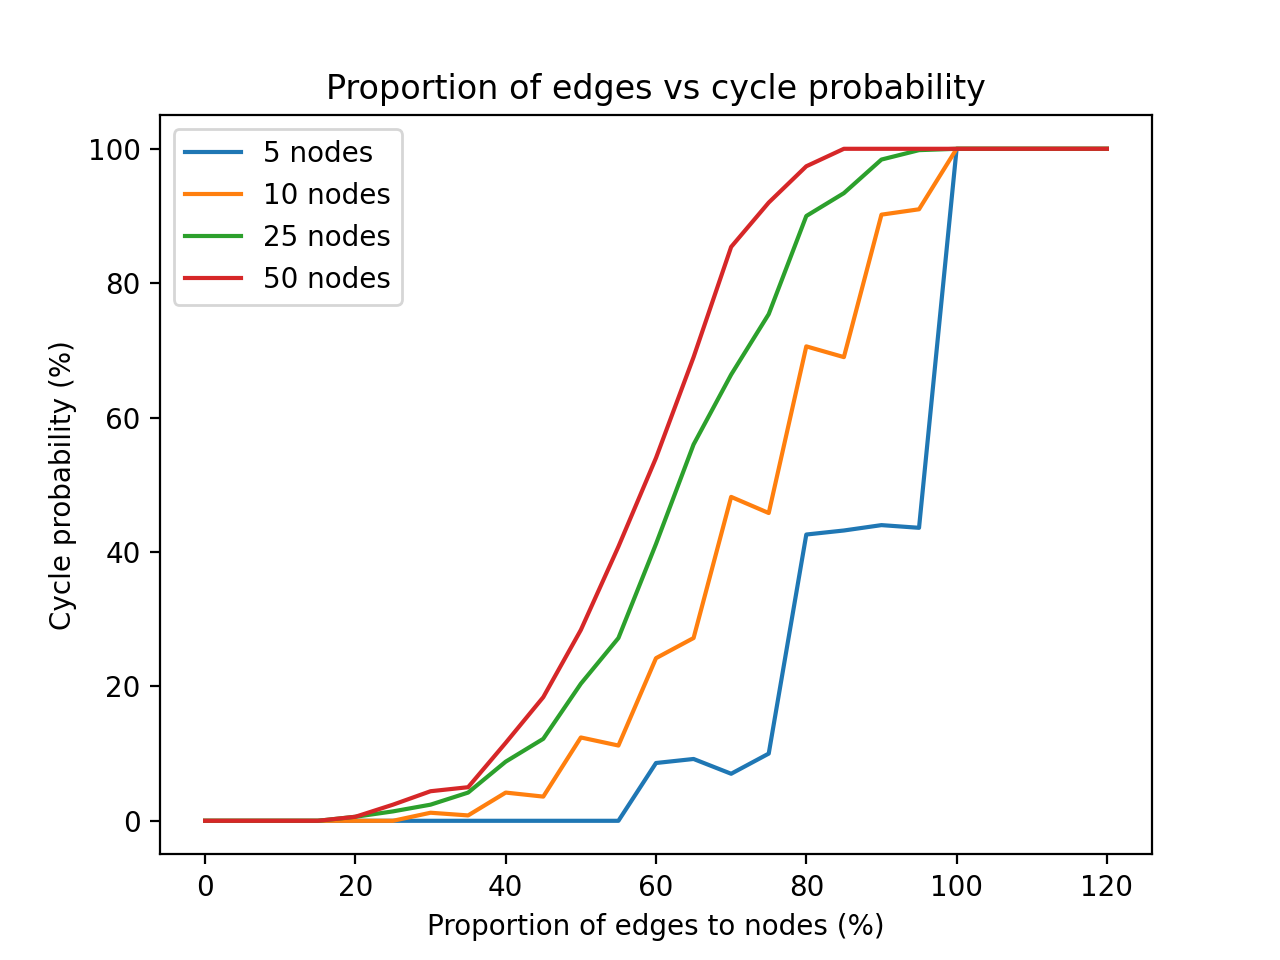
\includegraphics[width=0.8\linewidth]{experiment_1.png}
    \caption{Proportion of edges vs cycle probability}
    \label{fig:edges_vs_cycle}
\end{figure}


\subsection{Experiment 2}

Experiment 2 examines the probability of a graph being connected as the proportion of edges increases.

We compute the approximate connected probability for a graph of $e$ edges and $n$ nodes by generating 500 random graphs with $e$ edges and $n$ nodes and determining what percentage of those graphs are connected.

This process is conducted for graphs with 5, 10, 25, and 50 nodes at different proportions of edges. Specifically, we start with 0 edges and gradually increase to the maximum number of unique edges for the node count ($\sum_{i=0}^{n-1}i$) in 4\% steps, with 100\% being the maximum number of edges.

The result is then graphed as shown in Figure \ref{fig:edges_vs_connected} below.

\begin{figure}[H]
    \centering
    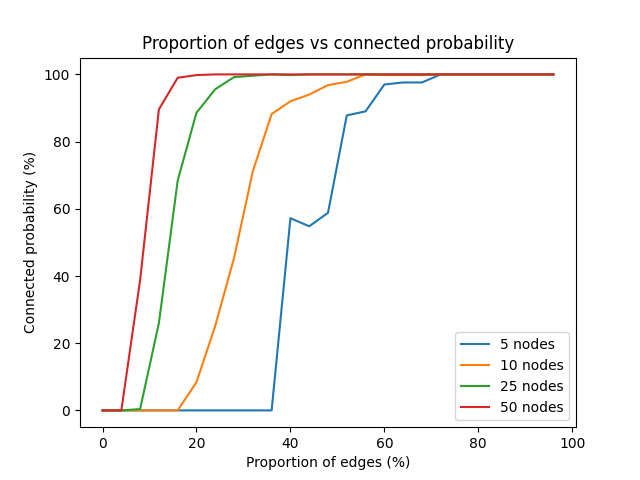
\includegraphics[width=0.8\linewidth]{experiment_2.png}
    \caption{Proportion of edges vs connected probability}
    \label{fig:edges_vs_connected}
\end{figure}

As seen in Figure \ref{fig:edges_vs_connected}, each graph size sits at a 0\% chance of connectedness before rapidly increasing and eventually reaching a 100\% probability of being connected; but the transitions take place at different edge proportions.

This is because the number of edges required to make connectedness possible grows linearly with the number of nodes, while the maximum number of unique edges grows quadratically. Specifically, an undirected graph of $n$ nodes with no self-loops requires only $n - 1$ unique edges to make connectedness possible, but can have a maximum of $\frac{(n - 1) \cdot n}{2}$ unique edges.

\section{Part 2}



\appendix
\section{Navigating the Code}

\begin{itemize}
    \item Each experiment can be found within it's own \verb|.py| or \verb|.ipynb| file titled \verb|experiment_#|
    \item Additional graph functions were added to \verb|graph.py|
\end{itemize}

\end{document}
